\newpage
\section{MIDI Equipment}
\subsection{MIDI Signal Path}

\begin{figure*}[h]
\centering
\includegraphics[width=.85\textwidth]{Images/BlockDiagramMIDI.png}
\caption{Block Diagram of MIDI Signal Path}
\label{fig:fullfig}
\end{figure*}

\subsection{Yamaha Clavinova CLP-50}

The Yamaha Clavinova CLP-50 is used as the MIDI controller in the MIDI Lab. It is used to control the other synthesizers and the DAW. By default the keyboard plays sound through its built in speaker. To turn this off, turn local off. \\

\textbf{To Turn Local Off} 

\begin{enumerate}
	\item Press and hold [TRANSPOSER]
	\item While holding [TRANSPOSER], press [PIANO NORMAL]	
\end{enumerate}

\newpage

\subsection{MOTU MIDI Time Piece MTP AV}
The Mark of the Unicorn MIDI Time Piece allows for MIDI communication between the MIDI controller (Yamaha Clavinova), the iMac, and the other synthesizers in the MIDI lab. \\

\begin{figure*}[h]
\centering
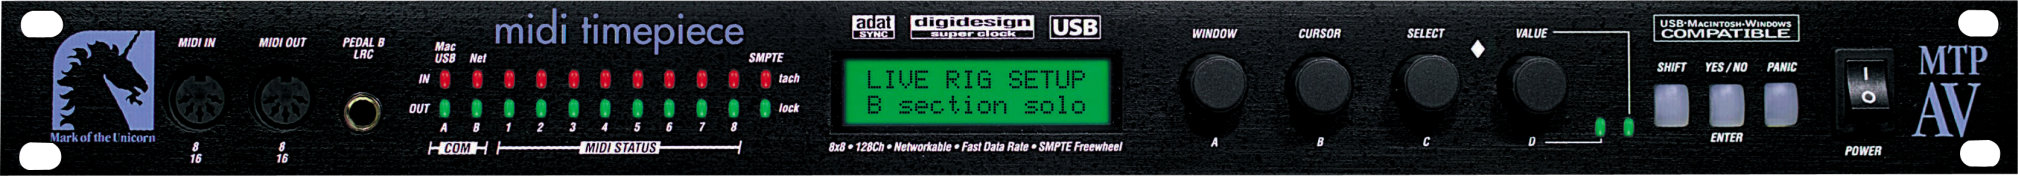
\includegraphics[width=.85\textwidth]{Images/MOTU.jpg}
\caption{MOTU MIDI Time Piece MTP AV}
\label{fig:fullfig}
\end{figure*}

\textbf{Control other synths using Yamaha Clavinova}
\begin{enumerate}
	\item Turn the [VALUE] knob until desired synth is selected (Computer, Korg Triton, Roland D-50,  E-mu Proteus 2000)
	\item Select the synth using the [YES/NO ENTER] button
\end{enumerate}

\textbf{Send MIDI from DAW to Synth}
\begin{enumerate}
	\item In chosen DAW create a MIDI channel 
	\item Have the MIDI To send to "MIDI Timepiece Port 1" for the Korg Triton, "MIDI Time Piece Port 2" for the Roland D-50, and "MIDI Time Piece Port 3" for the E-mu Proteus 2000. 
\end{enumerate}